\documentclass[10pt,a4paper]{article}
\usepackage[latin1]{inputenc}
\usepackage{amsmath}
\usepackage{amsfonts}
\usepackage{amssymb}
\usepackage{color}
\usepackage{graphicx}
\usepackage{hyperref}
\usepackage{enumitem}
\usepackage{graphicx}
\usepackage{array}
\usepackage{float}
\hypersetup{
	colorlinks=true,
	linkcolor=blue,
	filecolor=magenta,
	urlcolor=cyan,
}
\RequirePackage[left=01.1cm,top=3cm,right=1.5cm,bottom=2.5cm,nohead,nofoot]{geometry}


\newcolumntype{C}[1]{%
	>{\vbox to 2.5ex\bgroup\vfill\centering\arraybackslash}%
	p{#1}%
	<{\vskip-\baselineskip\vfill\egroup}}  

\author{\vspace{0.4cm}
	Anirudh N J \\\vspace{0.4cm}
	Somesh Devagekar \\\vspace{0.8cm}
	Raina Thomas}

\title{
	\vspace*{5cm}
	\textbf{Scientific Experimentation and Evaluation}
	}
	
\date{\color{blue}April 10, 2019}			
\begin{document}
	
\begin{titlepage}

	\maketitle
	
\end{titlepage}

\Large\textbf{\color{blue}LEGO NXT Project Implementation}

\Large
\begin{enumerate}[label=\Roman*]

\item
\vspace{0.5cm}
\Large{\textbf{Aim}}\\

The aim of this project is to construct a LEGO NXT differential drive robot and measure the observable end pose variation for three different trajectories: an arc to the left, driving straight and an arc to the right.
\vspace{0.5cm}

The experiment of measuring the end pose was done by measuring the pose using markers and Computer Vision.
   

\vspace{0.5cm}
\item
\Large{\textbf{Experimental Setup}}\\

\begin{enumerate}
	
	\item
	\textbf{Software Setup}\\
	
	\begin{enumerate}[label=(\roman*)]
		\item
		\textbf{Software Installation}\\
		
		The following softwares were installed in the PC for driving the robot :
			\vspace{0.3cm}
			\begin{enumerate}[label=(\alph*)]
				
				\item
				Java SE Development Kit 8 was installed in the Windows Operating System of the PC. The software was downloaded from the website :\\ \href{https://www.oracle.com/technetwork/java/javase/downloads/jdk8-downloads-2133151.html}{https://www.oracle.com}
				\vspace{0.2cm}
				
				\item
				Eclipse IDE for Java Developers was downloaded and installed from the website 
				\href{http://eclipse.bluemix.net/packages/neon/?JAVA-WIN32}{http://eclipse.bluemix.net}. This IDE is the platform used for developing the program for driving the robot.
				\vspace{0.2cm}
				
				\item
				The leJOS NXT Fantom Driver was downloaded from  \href{https://www.lego.com/en-us/mindstorms/downloads}{https://www.lego.com/en-us/mindstorms/download}. 
				\vspace{0.2cm}
				
				\item
				The leJOS NXJ software was downloaded from \href{https://sourceforge.net/projects/nxt.lejos.p/files/}{https://sourceforge.net} and installed in the PC using the Windows Installer.
				\vspace{0.2cm}
				
				\item
				The leJOS NXJ plug-in was added to Eclipse.
				\vspace{0.5cm}
								
			\end{enumerate}
			
			\item
			\vspace{0.2cm}
			\textbf{Programming the robot}\\
			\begin{enumerate}[label=(\alph*)]
				\item
				The Lego NXT Java template code provided in the website below was modified for use in the robot.
				\href{https://lea.hochschule-bonn-rhein-sieg.de/ilias.php?ref_id=571436&cmd=view&cmdClass=ilrepositorygui&cmdNode=t3&baseClass=ilrepositorygui}{https://lea.hochschule-bonn-rhein-sieg.de}
				\item
				A LeJOS NXT Project was created in Eclipse and the template code was added to the project and certain parameters in the code was modified. The parameters that were modified for our experimental setup are given in the table below.				
					
				\begin{table}[ht]				
					\centering
				\begin{tabular}{ | C{3cm} | C{3cm}|  C{7cm} |} 
					\hline
					\textbf{Parameter} & \textbf{Value} & \textbf{Reason}\\ 
					\hline
					SLEEP\_TIME   & 3000.0 &  Increased to make the robot drive for a longer duration\\ 
					\hline
					TURN\_RATE  & 10.0 & Decreased to prevent the robot from making sharp turns\\ 
					\hline
				\end{tabular}
					\caption{Modified Code Parameters}
				  	\label{Tab:Tcr}
				\end{table}
		\item
		The NXT Device was connected to the PC via a USB Cable.	The modified code was compiled and run as an LeJOS NXT Program to create a .nxj file. This was automatically flashed into the NXT device that was connected to the PC.
				
				
			\end{enumerate}
			
			
	\end{enumerate}

	
	\vspace{0.3cm}
	
	\item
	\Large{\textbf{Hardware Setup}}\\
	
To reproduce the above experiment the following equipment are needed :
\begin{enumerate}
    \item
    White A0 Grid Sheet
    \item
    Camera - Microsoft 
    \item
    Assembled robot - Lego NXT 
    \item
    Scales for measuring the length 
    \item
    Vision markers
\end{enumerate}
\vspace{0.5cm}

The general steps to setup the experiment are as following :
\begin{enumerate}
    \item
    Place the White A0 sheet on a flat surface.  Try to remove any bends in the sheet and keep the paper as flat as possible. This will be called the 'map' on which the robot will move on. The measurement system is made of the robot, scale, camera, aruco markers and a paper. 
    \item
    Draw the template drawing of the "floor space" taken by the robot as shown in the figure. Concept of "Behavior-shaping constraint" is used to prevent wrong initial placement of the robot.
    
    
    \begin{figure}[H]
	\centering
    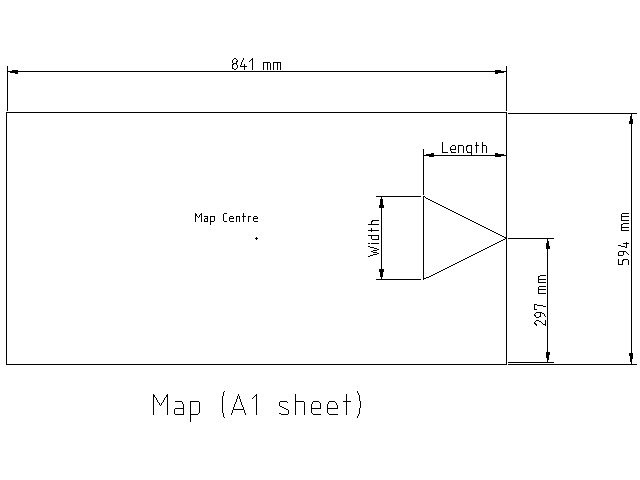
\includegraphics[width=0.6\linewidth ]{Template.png}
    \caption{ Template drawing of the Map along with dimensions}
    \end{figure}

	\item
	Four aruco markers of different ids are used to find the corners of the grid sheet. The aruco markers are aligned such that the first corner of the marker which is detected by the CV algorithm overlaps with the corner of the sheet.
	\item
	The markers are also aligned to be perfectly parallel to the sheet edges. These markers should be aligned properly since the next preprocessing steps are dependant on this.
	\item
	The camera is placed rigidly such that the whole sheet is visible and the centre of the camera points approximately to the centre of the sheet.	
    \item
    The robot was assembled using the manual given with the LEGO NXT box. The robot firmware was flashed as given in the Software Setup. 
    \item
    We assumed that the driving axle is towards the front(leading edge) of the robot and that the robot origin lies in the centre of the driving axle.
    \item
    Place the robot on the A0 sheet over the marked template.
    \item
	The measurands are the initial and end positions and the angles between the center of the robot and the tail of the robot.
    
\end{enumerate}
\vspace{0.5cm}

The reference images of the DUT and the proposed marker tracking visualization are given below.

\begin{figure}[h]
	\centering
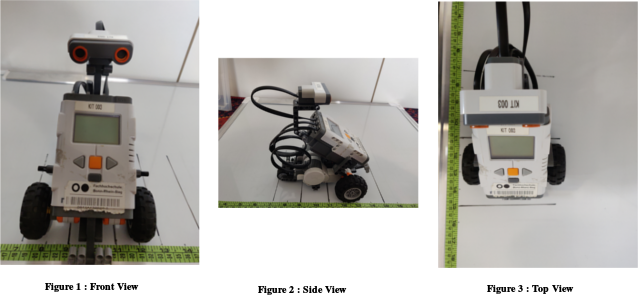
\includegraphics[width=0.9\linewidth ]{pose.jpeg}
\caption{ Views of the DUT}
\end{figure}


\end{enumerate}
\vspace{0.5cm}
\newpage
\item
\Large{\textbf{Procedure}}\\

\begin{enumerate}
	\item
	\Large{\textbf{Experimental Steps}}\\
	
\begin{enumerate}
	\item
	For this experiment the camera should be placed rigidly directly above the experiment setup such that the full map is visible in the camera frame. 
	\item
	Before beginning the experiment the camera should be calibrated and the obtained parameters should be used to compensate for the lens distortion and other errors in the image. 
	\item
	Two small markers should be attached on the flat surface of the robot, one on the front and one on the rear of the robot. The markers should be visible in the camera frame captured by the overhead camera. (The two markers should have different ID to distinguish between them)
	\item
    Using Computer-vision the two markers on the robot can be tracked and localized. The centre of the markers can be found and be used to calculate the offset from the actual robot origin using a scale or any other measuring device.
	\item
	The robot is programmed to move using the initial pose and the desired final pose.
	\item
	The initial pose and the final pose can be found by CV and position and pose in the required form can be extracted.
	\item
	20 measurements would be performed for each trajectory. Mean and standard deviation will be computed from the measurement. These measured values would be used to compute the accuracy and precision of the pose variation. 
	
\end{enumerate}

\vspace{0.5cm}

\begin{figure}[h]
	\centering
	
\includegraphics[width=0.2\linewidth ]{marker.png}
	\caption{ Example Aruco marker for computer vision}
\end{figure}


\item
\Large{\textbf{Computer Vision Algorithm}}\\
\begin{enumerate}[label=\roman*)]
		\item
		Preprocessing the image involves the following steps :
		\vspace{0.2cm}
		\begin{enumerate}[label=\alph*)]
			\item
			Camera calibration is done to find the intrinsic and extrinsic parameters of the camera.	These parameters are then used to remove the radial distortion from the image.
			\item
			The aruco markers on the four corners are then used to perform perspective transformation. This helps in removing minor skews in the image.
			\item
			Using the four corners of the sheet, the area of the sheet is cropped.			
		\end{enumerate}
		\vspace{0.3cm}
		\item
		Using the preprocessed image, the algorithm tries to find the two aruco markers that are placed on the robot.
		\item
		Using geometric calculations, the center of the aruco markers on the robots are found. 
		\item
		The marker positions are in pixels since it is directly calculated from the image. A transformation is performed on the pixel coordinates to convert it into 'millimeter' coordinates of the map.
		\item
		The scripts that were written for the experiment along with the documentation of each of the function are given in the following repository. (\href{https://github.com/njanirudh/SEE-Project}{https://github.com/njanirudh/SEE-Project})
\end{enumerate}



\end{enumerate}

\item
\vspace{0.5cm}
\textbf{Observations}\\

\textbf{Problems}

\begin{enumerate}
	\item
	This experiment accuracy and precision depended on the following aspects:
	\begin{enumerate}
		\item
		Camera Setup with respect to the grid sheet
		\item
		Lighting conditions
		\item
		Image recognition algorithms
	\end{enumerate}	 
	\item
	The robot deviated from the expected trajectory towards the left due to the following reasons:
	\begin{enumerate}
		\item
		Uneven weight distributions of the robot
		\item
		Difference in the tractions
		\item
		Faster rotation of one motor compared to the other
	\end{enumerate}
	\item
	Difference in the starting position of the robot during the experiment caused variations in the end pose of the robot.
	\item
	Mechanical adjustments performed on the DUT during the ecperiment affected the end poses.
	\item
	Errors that occured due to the markers are given below:
	\begin{enumerate}[label=(\roman*)]
		\item
		The marker placed at the front of the robot gets hidden at times when the robot moves to the left. This prevents the camera from detecting the marker.
		
		\vspace{0.5cm}
		
		\begin{figure}[h]
			\centering
			\includegraphics[width=0.35\linewidth ]{hidden_marker.png}
			\caption{ Hidden marker}
		\end{figure}
		
		\item
		The bounding box may not encompass the whole marker. This causes inaccurate calculation of marker centers.
		
		\vspace{0.5cm}
		
		\begin{figure}[H]
			\centering
			\includegraphics[width=0.35\linewidth ]{marker_detection_error.png}
			\caption{Bounding Box Error}
		\end{figure}
		
		\item
		The marker in the image appears skewed, which results in inaccurate calculation of pose.
		
		\begin{figure}[H]
			\centering
			\includegraphics[width=0.45\linewidth ]{skew.png}
			\caption{Skewed Marker}
		\end{figure}
		
		
	\end{enumerate}
	
	
\end{enumerate}
\newpage
\vspace{0.5cm}

\vspace{0.5cm}
\textbf{Data Visualisation}\\

The origin of the original map (grid sheet) that was considered was at the top-left corner. However, the plots that have been displayed in this section have the origin in the bottom-left corner and hence the original images have been mirrored to fit the plot axes.

\begin{enumerate}
	\item
	The scatter plot of the initial pose of the robot has been displayed in the figure below.

\begin{figure}[H]
	\centering
	\includegraphics[width=0.9\linewidth ]{front.png}
	\caption{Initial Pose}
\end{figure}

\newpage
\item
The scatter plot of the end pose of the robot after it moved forward has been displayed in the figure below.

\begin{figure}[H]
	\centering
	\includegraphics[width=0.9\linewidth ]{forward.png}
	\caption{End Pose - Forward}
\end{figure}

\newpage
\item
The scatter plot of the end pose of the robot after it moved in the left arc has been displayed in the figure below.

\begin{figure}[H]
	\centering
	\includegraphics[width=0.9\linewidth ]{left.png}
	\caption{End Pose - Left}
\end{figure}


\newpage
\item
The scatter plot of the end pose of the robot after it moved in the right arc has been displayed in the figure below.

\begin{figure}[H]
	\centering
	\includegraphics[width=0.9\linewidth ]{right.png}
	\caption{End Pose - Right}
\end{figure}

\end{enumerate}

\end{enumerate}






\end{document}


